% Creating a simple Title Page in Beamer
\documentclass[aspectratio=169]{beamer}
\usepackage{tikz}
\usepackage{tikz-uml}
\usetikzlibrary{shapes}
\usetikzlibrary{arrows}      % use arrow with 90°
\usetikzlibrary{arrows.meta}      % use arrow with 90°
\usetikzlibrary{calc}        % compute midpoint $(A)!0.5!(b)$
\usetikzlibrary{fit}        % fit several nodes
\usetikzlibrary{backgrounds}        % fit several nodes
\usetikzlibrary{positioning}  % of left = of {1cm} NODE
\usetikzlibrary{automata} % draw finite automata
\usetikzlibrary{decorations.markings}
\usetikzlibrary{decorations.pathreplacing} %%curly braces
\usetikzlibrary{decorations.pathmorphing} %% snake, saw
\usetikzlibrary{decorations} %%curly braces
\usetikzlibrary{quotes} %%curly braces
\usetikzlibrary{intersections} % intersections
\usetikzlibrary{patterns}      % fill nodes with pattersn
\usetikzlibrary{tikzmark}      % fill nodes with pattersn

\usepackage{media9}
\usepackage{hyperref}
\usepackage{fancyvrb}
\usepackage{graphicx} % Required to include images
\usepackage{inconsolata}
\usepackage{listings}
\usepackage{balance}
\usepackage{booktabs}
\usepackage[cal=boondox]{mathalfa}
\usepackage[english]{babel}
\usepackage{amssymb}% math symbols as mathbb, \mathsf{d}
\usepackage{amsmath}
\usepackage{amsthm}
\usepackage{mathrsfs}
\usepackage{siunitx} %units
\usepackage{enumerate}
\usepackage{graphicx}
\usepackage{soul}
\usepackage{tabularx}
\usepackage{siunitx}
\usepackage{array}
\normalfont%
\usepackage[T1]{fontenc}
\usepackage{textcomp}
\usepackage{tikz}
\usetikzlibrary{patterns}
\usepackage[utf8]{inputenc}
\usepackage{tikz-cd} % commutative diagrams with tikz
\usepackage[ruled,vlined,linesnumbered]{algorithm2e}
\SetKw{KwTo}{To}
\SetKwRepeat{Do}{do}{while}
\usepackage{caption}
\usepackage{subcaption}

\def\WP{{\mathit{VP}}}
\def\d{\mathsf{d}}
\def\pathv{\mathbf{p}}
\def\path{p}
\def\Rn{\mathbb{R}^n}
\def\R{\mathbb{R}}
\def\Lcal{\mathcal{L}}
\def\Lcalsharp{\mathcal{L}^\#}
\def\Fcal{\mathcal{F}}
\def\Gcal{\mathcal{G}}
\def\Acal{\mathcal{A}}
\def\Mcal{\mathcal{M}}
\def\Ocal{\mathcal{O}}
\def\Ocalfree{\mathcal{O}_{\text{free}}}
\def\Sob{\mathbb{W}^{k,2}}
\def\hatL{\hat{L}}
\def\sinv{s^{-1}}

\newcommand\diff[2]{\frac{\d #1}{\d #2}}
\newcommand\diffp[2]{\frac{\partial{} #1}{\partial{} #2}}
\newcommand\diffk[3]{\frac{\d^{#3} #1}{\d #2^{#3}}}

\def\Fqi{F\big(\qv_i, \dot{\qv}_i,\ddot{\qv}_i\big)}
\def\Gci{G_i\big(\qvnom, \dot{\qvnom},\ddot{\qvnom}\big)}

\def\xiinv{\xi^{\text{-}1}}
\def\diffeo{\text{-Diffeo}}
\newcommand\Ckdiffeo[1]{C^{#1}\text{-Diffeo}}

\newcommand\scaleddot{\scalebox{.89}{.}}
\makeatletter
\renewcommand{\dddot}[1]{%
	{\mathop{\kern\z@#1}\limits^{\makebox[0pt][c]{\vbox to-1.5\ex@{\kern-\tw@\ex@
						\hbox{\normalfont\scaleddot\kern-0.5pt\scaleddot\kern-0.5pt\scaleddot}\vss}}}}}
\renewcommand{\ddddot}[1]{%
	{\mathop{\kern\z@#1}\limits^{\makebox[0pt][c]{\vbox to-2.2\ex@{\kern-\tw@\ex@
						\hbox{\normalfont\scaleddot\kern-0.5pt\scaleddot\kern-0.5pt\scaleddot\kern-0.5pt\scaleddot}\vss}}}}}
\makeatother

\def\qvnom{\mathbf{p}}
\def\qnom{p}
\def\Jnom{J'}
\def\Tnom{\mathcal{T}}
\def\tnom{\tau}

\def\psibf{\pmb{\psi}}
\def\chibf{\pmb{\chi}}

\def\qv{\mathbf{q}}
\def\Qv{\mathbf{Q}}
\def\wp{\mathbf{w}}
\def\kv{\mathbf{k}}
\def\pv{\mathbf{p}}
\def\Fv{\mathbf{F}}
\def\Bv{\mathbf{B}}
\def\yv{\mathbf{y}}
\def\Pv{\mathbf{P}}
\def\vv{\mathbf{v}}
\def\cv{\mathbf{c}}
\def\dv{\mathbf{d}}
\def\ev{\mathbf{e}}
\def\bv{\mathbf{b}}
\def\xv{\mathbf{x}}
\def\uv{\mathbf{u}}
\def\zv{\mathbf{z}}
\def\av{\mathbf{a}}
\def\Tv{\mathbf{T}}
\def\mv{\mathbfcal{m}}
\def\basis{\mathbfcal{B}}
\def\nv{\mathbfcal{n}}
\def\Nv{\mathbfcal{N}}
\def\Ev{\mathbfcal{E}}
\def\pv{\mathbfcal{p}}
\def\mvi{\mathcal{m}}
\def\nvi{\mathcal{n}}
\def\Nvi{\mathcal{N}}
\def\pvi{\mathcal{p}}
\def\Evi{\mathcal{E}}

\def\rv{\mathbf{r}}
\def\wv{\mathbf{w}}
\def\xv{\mathbf{x}}
\def\hv{\mathbf{h}}
\def\hmu{{\hat{\mu}}}
\def\hxi{{\hat{\xi}}}
\def\calT{{\mathcal{T}}}



\def\Dbf{\mathbf{D}}
\def\Abf{\mathbf{A}}
\def\Bbf{\mathbf{B}}
\def\Cbf{\mathbf{C}}
\def\Nbf{\mathbf{N}}
\def\Ebf{\mathbf{E}}

\def\dint{{\d_{\text{inn}}}}
\def\dtot{{\d^{\text{*}}}}
\def\dgen{{\d^{\text{*}}}}
\def\piv{\boldsymbol{\pi}}
\def\kappav{\boldsymbol{\kappa}}



\def\Nop{\mathbf{N}}

\def\hNop{\hat{\mathbf{N}}}
\def\hatN{\hat{N}}
\def\hatNv{\hat{\mathbf{N}}}
\def\hatE{\hat{E}}
\def\hatEv{\hat{\mathbf{E}}}

\def\nc{{n_c}}

\def\diffeo{\text{Diffeo}}

\def\Qsc{\mathscr{Q}}

\def\viso{v_{\text{\tiny max}}}
\def\qpmax{v_{q}}
\def\qppmax{a_{q}}

\def\eop{\mathbf{\hat{e}}_{o}}
\def\vop{v_{\text{\tiny o}}}


\def\tauv{{\boldsymbol\tau}}
\def\chiv{{\boldsymbol\chi}}

\def\Tsafe{T_{\text{safe}}}

\def\bfD{\mathbf{D}}
\def\bfG{\mathbf{G}}
\def\bfQ{\mathbf{Q}}
\def\bfJ{\mathbf{J}}
\def\bfA{\mathbf{A}}
\def\bfS{\mathbf{S}}


\def\bigO{\mathcal{O}}
\def\r{r}
\def\dt{\delta t}
\def\dq{\delta{\qv}}
\def\dqd{\delta \dot{\qv} }
\def\dqdd{\delta \ddot{\qv}}



\def\e{\varepsilon}


\def\ia{{j_1}}
\def\ib{{i_b}}
\def\iba{{i_{b,1}}}
\def\ibb{{i_{b,2}}}
\def\ic{{j_3}}
\def\id{{j_4}}
\def\ie{{j_5}}
\def\iif{{j_6}}
\def\ig{{j_7}}
\def\ih{{j_8}}

\newcommand\DF{\mathit{DF}}

\newcommand{\warntext}[1]{\textcolor{orange}{#1}}
\definecolor{imfusionBlue}{HTML}{00b0db}
\newcommand{\emphImFusion}[1]{\textcolor{imfusionBlue}{#1}}




\lstset{language=c++,
	basicstyle=\fontsize{5pt}{0pt}\selectfont\fontfamily{zi4}\selectfont,
	keywordstyle=\color{blue}\ttfamily,
	stringstyle=\color{red}\ttfamily,
	commentstyle=\color{green}\ttfamily,
	morecomment=[l][\color{magenta}]{\#}
}
\definecolor{maroon}{rgb}{0.5,0,0}
\definecolor{darkgreen}{rgb}{0,0.5,0}
\lstdefinelanguage{XML}
{
	basicstyle=\fontsize{4pt}{0pt}\selectfont\fontfamily{zi4}\selectfont,
	morestring=[s]{"}{"},
	morecomment=[s]{?}{?},
	morecomment=[s]{!--}{--},
	commentstyle=\color{darkgreen},
	moredelim=[s][\color{black}]{>}{<},
	moredelim=[s][\color{red}]{\ }{=},
	stringstyle=\color{blue},
	identifierstyle=\color{maroon}
}


% Theme choice:
\usetheme{ImFusion}

% Title page details: 
\title{GSplines: An
	analytically and algebraically consistency library for motion planning and optimization}
\author{Rafael A. Rojas}
\date{\today}


\begin{document}

\frame{\titlepage}
\begin{frame}[t]
	\frametitle{Who we are?}
	\hglue -1cm
	\begin{tikzpicture}[scale=1, transform shape]
		\node (a) {
			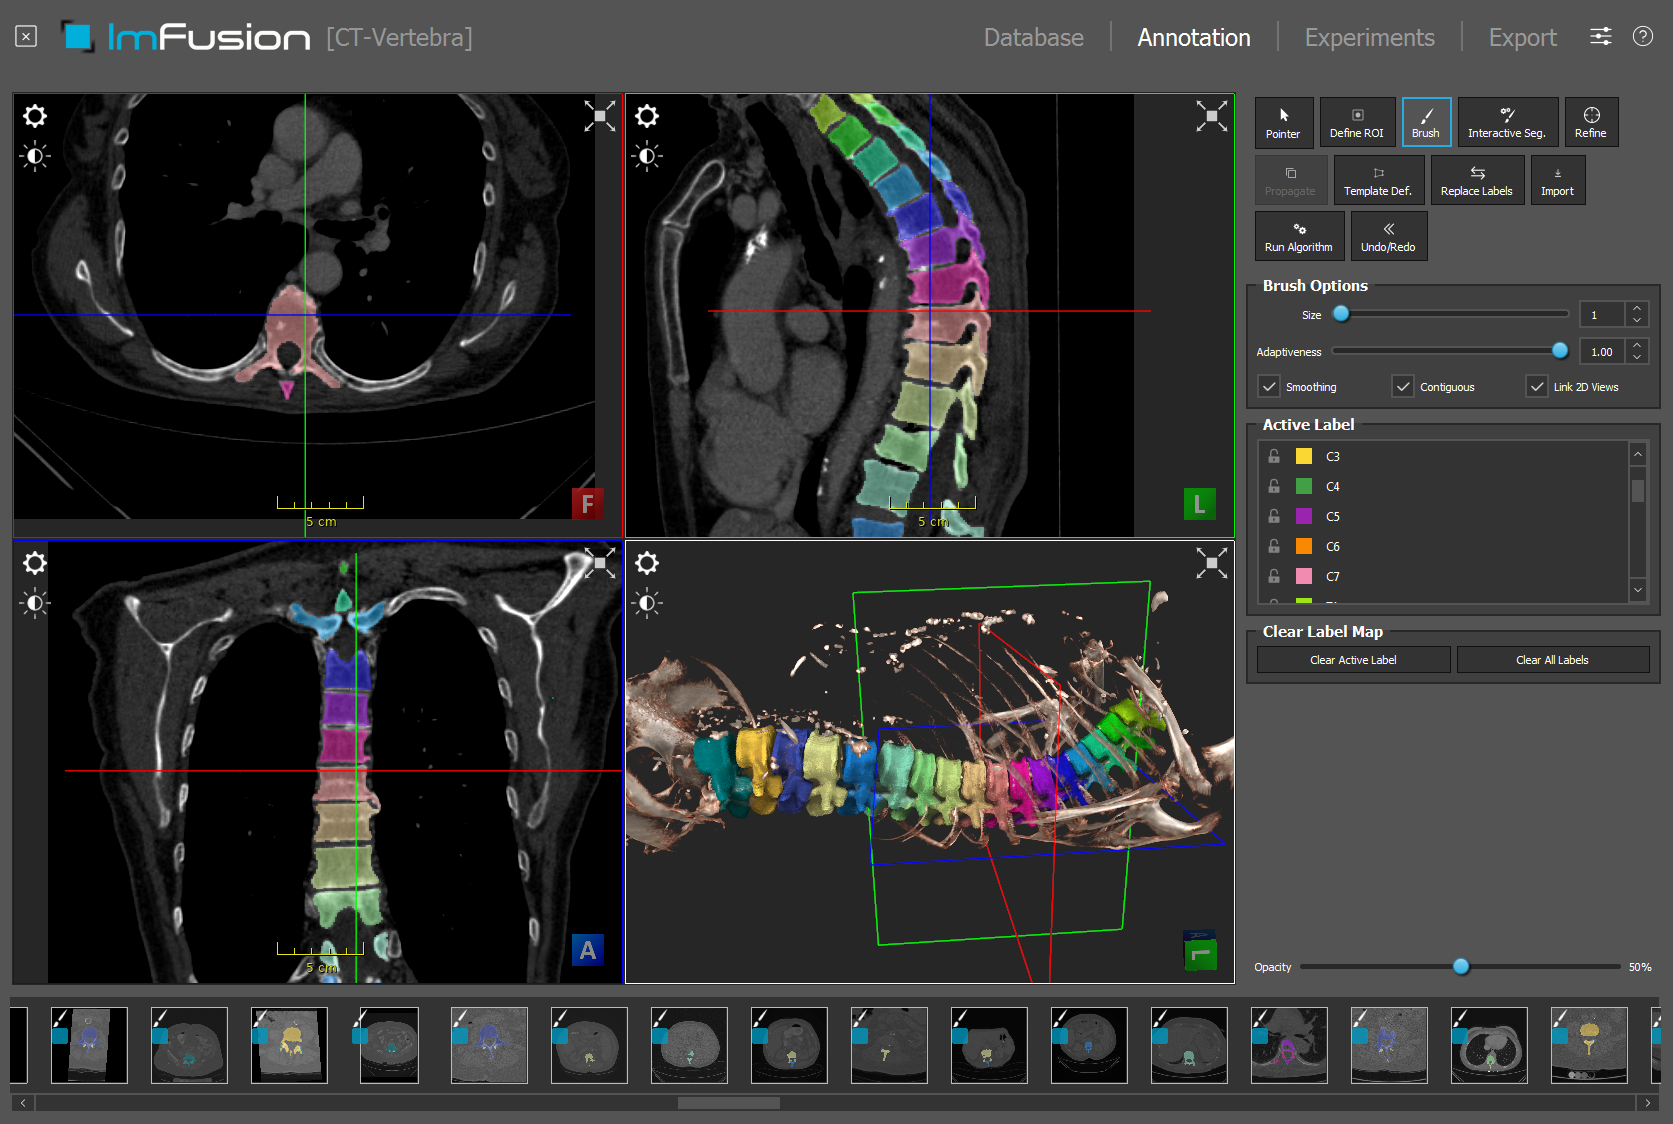
\includegraphics[width=2.5cm]{./images/imfusion_picture_00.png}};
		\node[anchor=north west] (box) at (a.north east) {
			\parbox{10cm}{%
				\begin{itemize}
					\item[{
\includegraphics[height=1.5ex]{./images/icon_place.png}}] Founded: 2012 | Location: Munich, Germany
					\item[{
\includegraphics[height=1.5ex]{./images/icon_flask.png}}] Private \& Independent R\&D Lab
					\item[{
\includegraphics[height=1.5ex]{./images/icon_handshake.png}}] Software framework: trusted by industry leaders, start-ups, and research labs
					\item[{
\includegraphics[height=1.5ex]{./images/icon_glass.png}}] Academic engagement: Actively contributing to the research community
					\item[{
\includegraphics[height=1.5ex]{./images/icon_group.png}}] Our team:
					\begin{itemize}
						\item 50+ dedicated employees and several students
						\item Global Diversity: 10+ Nationalities
						\item Excellence in Expertise: 50\% of technical staff hold a PhD
						\item Groups: Core, Computer Vision, Machine Learning, Ultrasound, CT \& Interventional X-Ray, Robotics.
					\end{itemize}
				\end{itemize}
			}
		};
		\node[anchor=north] at (a.south) {
			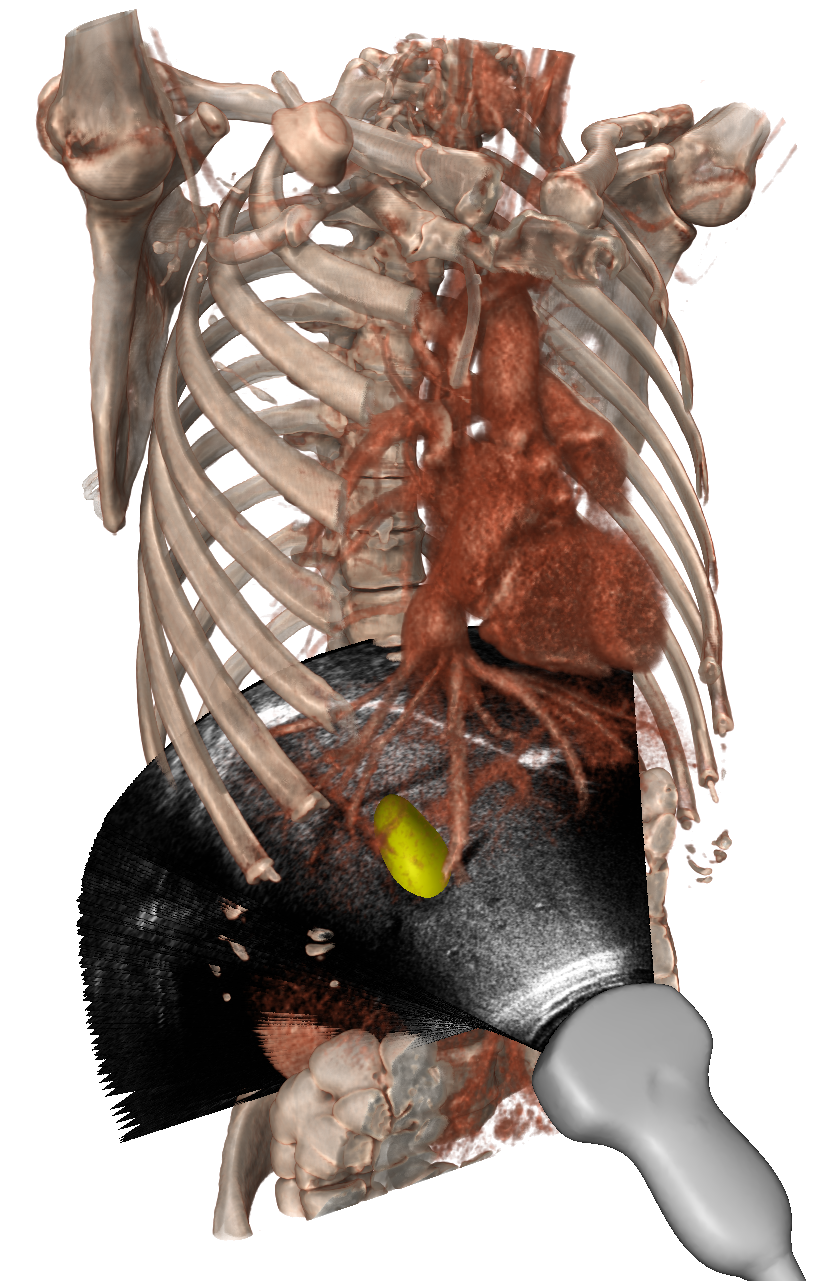
\includegraphics[width=2.5cm]{./images/imfusion_picture_01.png}};
		\node[anchor=north west] at (box.north east) {
			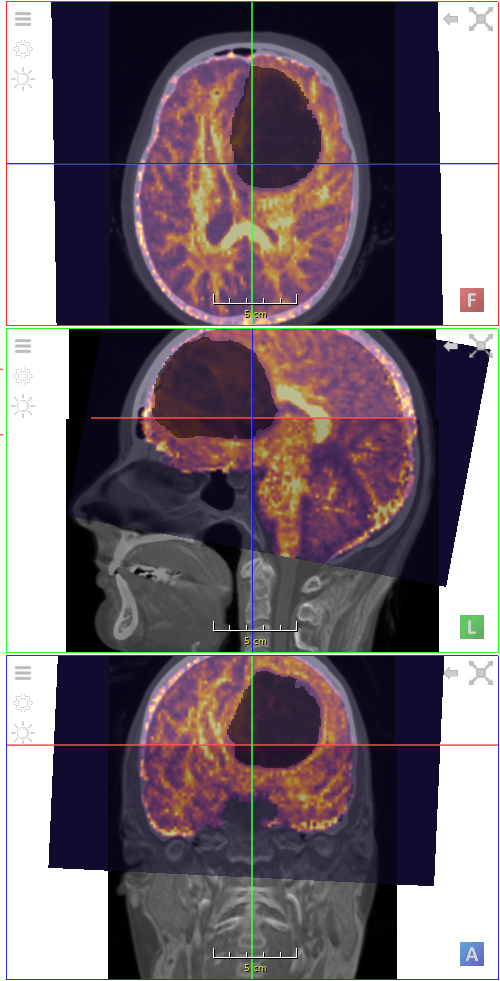
\includegraphics[width=2.5cm]{./images/imfusion_picture_02.png}};
	\end{tikzpicture}
\end{frame}

\begin{frame}[t]
	\frametitle{Robotics}
	\hglue -1cm
	\begin{tikzpicture}[scale=1, transform shape]
		\node (a) {
			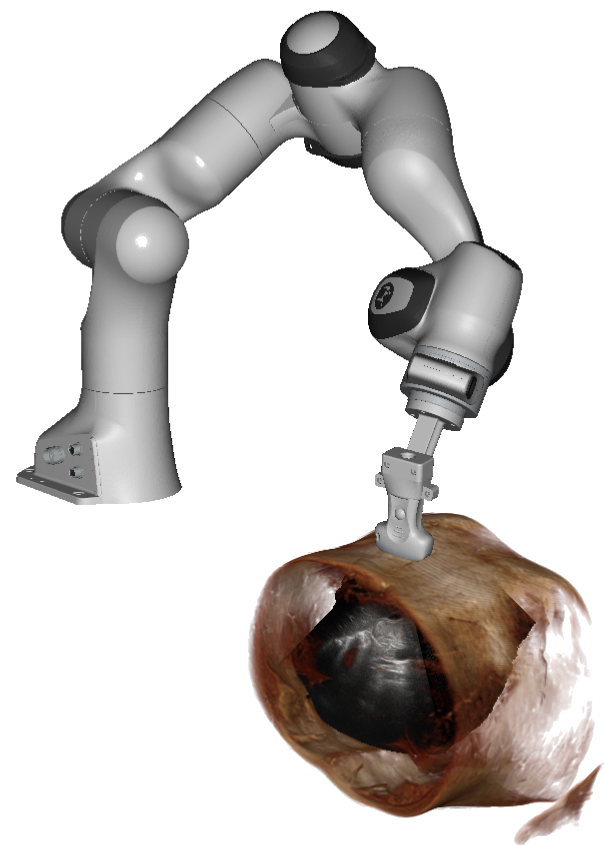
\includegraphics[width=3.4cm]{./images/imfusion_picture_03.png}};
		\node[anchor=north west] (box) at (a.north east) {
			\parbox{10cm}{%
				\begin{itemize}
					\item Deep integration with our framework for surgical navigation, freehand ultrasound, RGBD reconstruction, and more.
					\item Native support for popular robots: Franka Panda, Universal Robot UR-e series, Kuka
					\item Advanced utilities for key use cases: hand-eye calibration, object tracking, telerobotics, custom control strategies.
				\end{itemize}
			}
		};
	\end{tikzpicture}
\end{frame}

\section{Motivation}

\begin{frame}[t]
	\frametitle{Motivation: Academic Interest}

	{\fontsize{10}{6}
		\begin{columns}
			\begin{column}{0.5\textwidth}
				\begin{itemize}
					\only<1>{%
					\item {\bf Minimum Jerk} seems to be a thing
					      \begin{itemize}
						      \item Low frequency composition: low wear
						      \item Human-like motions: Flash and Hogan
						      \item Psychological safety
					      \end{itemize}
					      }
					      \only<2>{%
					\item Minimum Snap is of interest for drone motion planning
					      }
					      \only<3>{%
					\item Minimum-X
					      }
				\end{itemize}
			\end{column}
			\begin{column}{0.5\textwidth}
				\begin{center}
					\only<1>{
						\vskip-1cm
						\large
						\begin{equation*}
							\min  \int_0^T \left\|\diffk{\qv}{t}{3}\right\| \d t
						\end{equation*}
					}
					\only<2>{
						\large
						\begin{equation*}
							\min  \int_0^T \left\|\diffk{\qv}{t}{4}\right\| \d t
						\end{equation*}
					}
					\only<3>{
						\large
						\begin{equation*}
							\min  \int_0^T \left\|\diffk{\qv}{t}{X}\right\| \d t
						\end{equation*}
					}
					\begin{tikzpicture}
						\only<1>{
							\node[] (title) {%
								
\includegraphics[width=\textwidth]{./images/flashAndHoganTitle.png}
							};
							\node[anchor=north east] at (title.south east) {%
								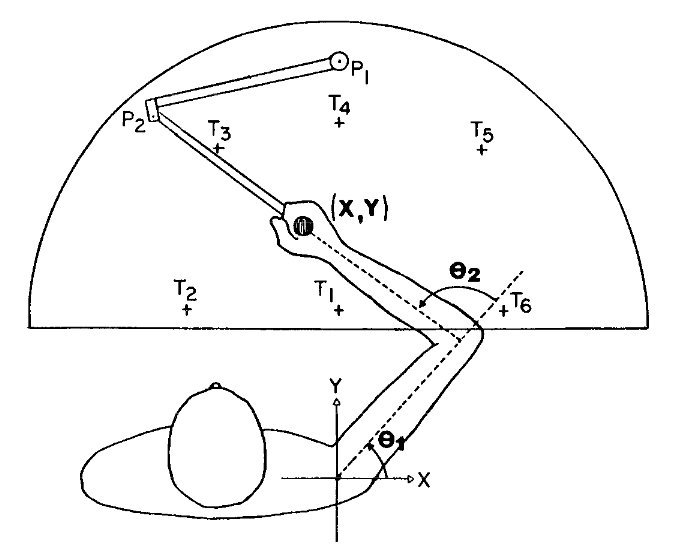
\includegraphics[width=0.3\textwidth]{./images/flashAndHoganExperiment.png}
							};
							\node[anchor=north west] (foo) at (title.south west) {%
								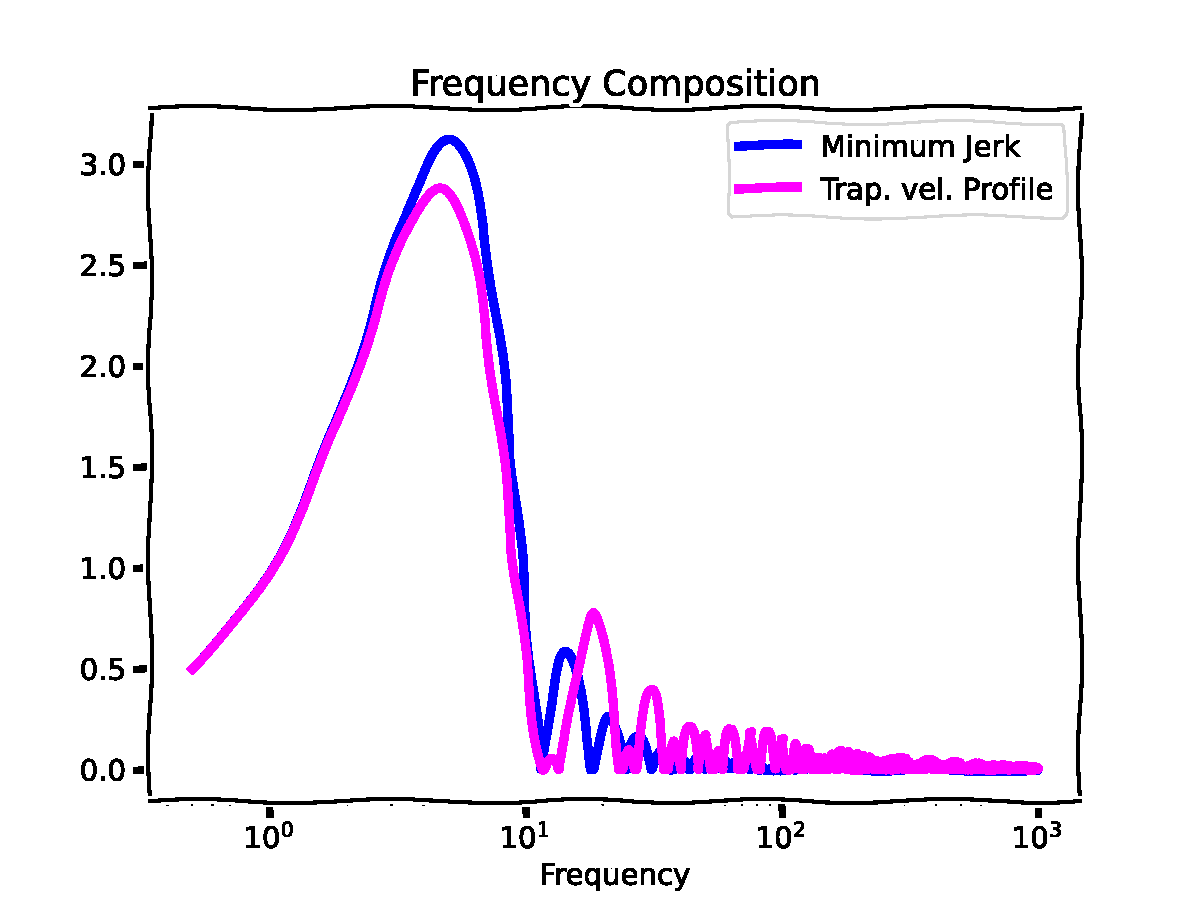
\includegraphics[width=0.3\textwidth]{./images/freq.pdf}
							};
							\node[anchor=north west] at (foo.south west) {%
								
\includegraphics[width=\textwidth]{./images/image27.png}
							};
						}
						\only<2>{
							\node[] (title) {%
								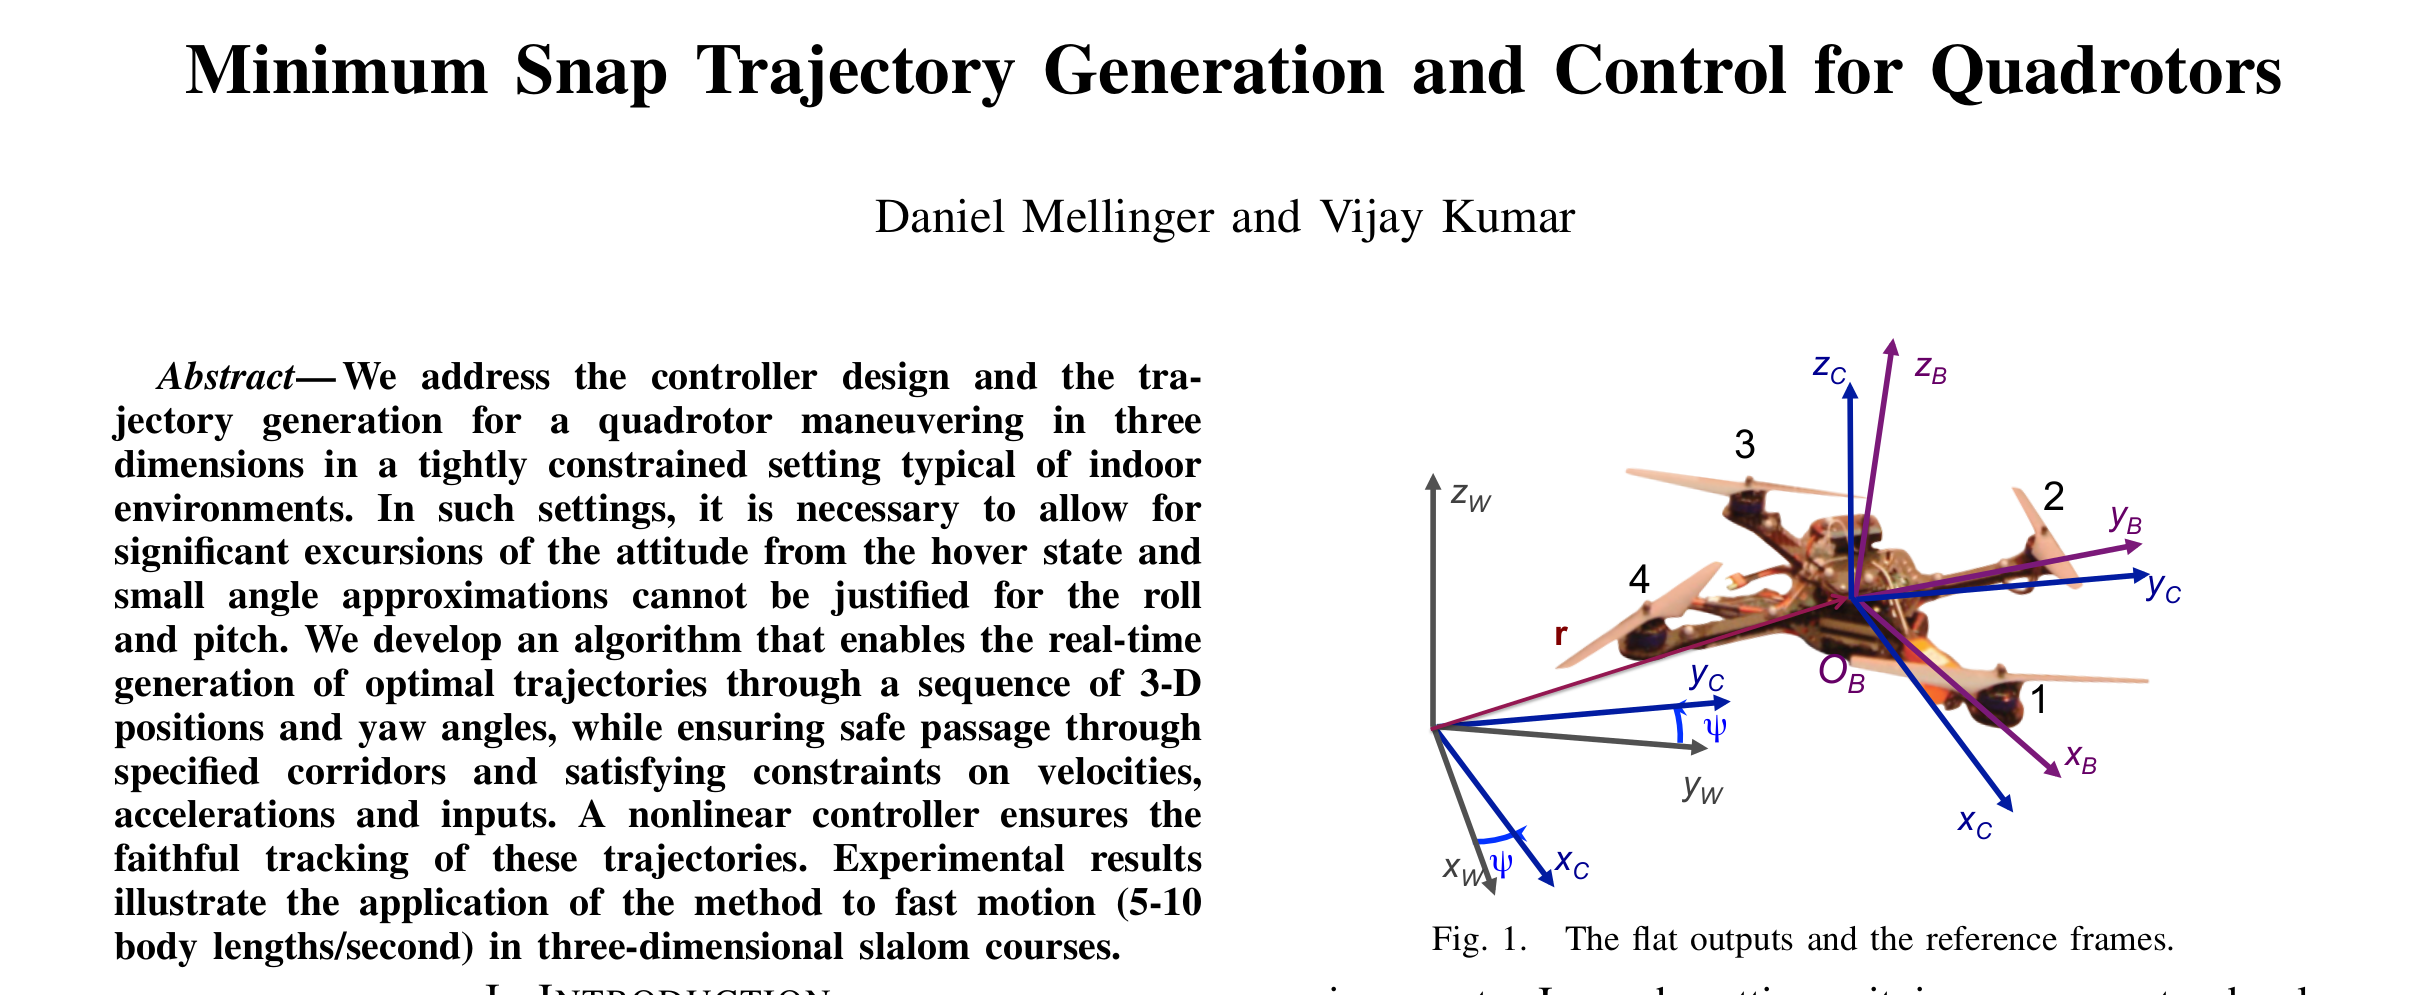
\includegraphics[width=\textwidth]{./images/mellingerKumarMinSnap.png}
							};
						}
					\end{tikzpicture}
				\end{center}
			\end{column}
		\end{columns}
	}
\end{frame}

\begin{frame}[t]
	\frametitle{Motivation: Output of Motion Planners}
	\begin{itemize}
		\item Sampled based \textbf{motion planners} generate waypoints that must be connected
		\item Lead-Through/Hand-Guiding programming of cobots
		      \includemedia[
			      width=0.6\linewidth,   % Adjust width
			      height=0.4\linewidth,  % Adjust height
			      activate=pageopen,      % Video starts on click
			      addresource=images/cobotWaypoints.mp4, % Path to the video
			      flashvars={source=images/cobotWaypoints.mp4&autoPlay=true&loop=true}
		      ]{}{VPlayer.swf}
	\end{itemize}
\end{frame}

\begin{frame}[fragile]
	\frametitle{Motivation: Current Classes Used in ROS Ecosystem}
	\begin{columns}
		\begin{column}{0.5\textwidth}
			\begin{itemize}
				\item Default ROS messages types for are defined as nested structrures.
				      The array-of-structures format leads to \emphImFusion{inefficient memory layout} and complicates the translation into the flat vector format that optimizers require.
				\item Other types are thighty coupled with the robot model
				\item do not provide clear interface for
				      \begin{itemize}
					      \item Evaluation at arbitrary time instantes
					      \item Computation of the derivatives
					      \item Time scaling
				      \end{itemize}
			\end{itemize}

		\end{column}
		\begin{column}{0.5\textwidth}
			Trajectory Message
			\begin{lstlisting}[basicstyle=\fontsize{5pt}{0pt}\selectfont\fontfamily{zi4}\selectfont]
std_msgs/msg/Header header
string[] joint_names
trajectory_msgs/msg/JointTrajectoryPoint[] points
            \end{lstlisting}
			Trajectory Point
			\begin{lstlisting}
double[] positions
double[] velocities
double[] accelerations
double[] effort
builtin_interfaces/msg/Duration time_from_start
                \end{lstlisting}
			Chomp trajectory
			\begin{lstlisting}
class ChompTrajectory
{
public:
...
    ChompTrajectory(const moveit::core::RobotModelConstPtr& robot_model, ...);
    double& operator()(size_t traj_point, size_t joint);
...
private:
...
    void init(); 
    std::string planning_group_name_;  
    Eigen::MatrixXd trajectory_;      
...
};
                \end{lstlisting}
		\end{column}
	\end{columns}
\end{frame}

\section{Goals}

\begin{frame}[t]
	\frametitle{Goals}

	\vfill
	{\fontsize{10}{6}
		Define class \texttt{GSpline} type that is capable of \emphImFusion{representing}:
		\begin{itemize}
			\item \emphImFusion{Solutions} of the generalized  Minimum-X problem: a \emph{convex} combination of norms of derivatives
			      \begin{eqnarray*}
				      &&\min \int_{t_0}^{t_f} \alpha_1 \left\|\diff{\qv}{t}\right\|^2 + \alpha_2 \left\|\diffk{\qv}{t}{2}\right\|^2 + \cdots  + \alpha_1 \left\|\diffk{\qv}{t}{k} \right\|^2 \d t \\
				      &&\qv(t_i) = \wp_i \ \ t_i\ \text{ is unknown}
			      \end{eqnarray*}
			\item The following \emphImFusion{transformations}
			      \begin{itemize}
				      \item Derivatives
				      \item Linear operations
				      \item Linear Scaling
			      \end{itemize}
			\item Available in \tikz[baseline]{\node{
\includegraphics[height=1cm]{images/python-logo-only.png}}} and \tikz[baseline=-1mm]{\node{
\includegraphics[height=1cm]{./images/c++logo.png}}}
			\item \emphImFusion{Remark:} This is not an alternative other general optimization tools like CASADI.
		\end{itemize}
	}
	\vfill
\end{frame}
\begin{frame}[t]
	\frametitle{Achieving Our Goal Through Variational Principles}

	We consider the problem of the minimization of a \emph{convex} combination of norms of the derivatives

	\begin{eqnarray*}
		&&\min \int_{t_0}^{t_f} \alpha_1 \left\|\diff{\qv}{t}\right\|^2 + \alpha_2 \left\|\diffk{\qv}{t}{2}\right\|^2 + \cdots  + \alpha_k \left\|\diffk{\qv}{t}{k} \right\|^2 \d t \\
		&&\qv(t_i) = \wp_i \ \ t_i\ \text{ is unknown!}
	\end{eqnarray*}

	Thanks to the \emphImFusion{Calculus of variations} we know that any minimizer solves the Euler-Lagrange equations

	\begin{equation*}
		-\alpha_1 \diffk{\qv}{t}{2}+ \alpha_2 \diffk{\qv}{t}{4}- \cdots +  {(-1)}^k \alpha_k \diffk{\qv}{t}{2k}= 0 \ \ \text{a.e.}
	\end{equation*}

\end{frame}

\begin{frame}[t]
	\frametitle{Achieving Our Goal Through Variational Principles}
	{\fontsize{9}{5}
		We call a \emphImFusion{\texttt{GSpline}} a solution of
		\begin{equation*}
			-\alpha_1 \diffk{\qv}{t}{2}+ \alpha_2 \diffk{\qv}{t}{4}- \cdots +  {(-1)}^k \alpha_k \diffk{\qv}{t}{2k}= 0 \ \ \text{a.e.}
		\end{equation*}
		Any \texttt{GSpline} Have the following properties
		\begin{itemize}
			\item Analytical Consistency
			      \begin{equation*}
				      \diffk{}{t}{k}:\text{GSpline}\longrightarrow \text{GSpline}
			      \end{equation*}
			\item Algebraic Consistency I
			      \begin{eqnarray*}
				      +:\text{GSpline}\times\text{GSpline}\longrightarrow \text{GSpline}\\
				      \cdot:\mathbb{R} \times \text{GSpline}\longrightarrow \text{GSpline}
			      \end{eqnarray*}
			\item Algebraic Consistency II
			      \begin{eqnarray*}
				      \left[t \rightarrow \sigma t \right]:\text{GSpline}\longrightarrow \text{GSpline}
			      \end{eqnarray*}
		\end{itemize}
	}
\end{frame}
\begin{frame}[t]
	\frametitle{Goals: Monoid property}
	\begin{itemize}
		\item We desire to achieve the monoid property on the derivative, scaling and addition/scalar multiplication operations. These operation will become a monoid under the composition.
		\item Composition is a fundamental tool in programming, the Monoid structure is the most fundamental compositional structure
	\end{itemize}
	\vskip 1cm
	\begin{center}
		
\includegraphics[height=0.2\textwidth]{./images/ccpconMonoids.png}
		
\includegraphics[height=0.2\textwidth]{./images/FunctionalProgrammingForDummies.jpeg}
		
\includegraphics[height=0.2\textwidth]{./images/categoryTheoryForProgrammers.jpg}
	\end{center}
\end{frame}


\section{Design}
\begin{frame}[fragile]
	\frametitle{Class Design: Solution Representation}


	\begin{tikzpicture}
		\node[anchor=north west] at (-1, 4){%
			\parbox{10cm}{%
				\small
				The solution of the corresponding Euler-Lagrange equations
					{%
						\begin{equation*}
							-\alpha_1 \diffk{\qv}{t}{2}+ \alpha_2 \diffk{\qv}{t}{4}- \cdots +  {(-1)}^k \alpha_k \diffk{\qv}{t}{2k}= 0 \ \ \text{a.e.}
						\end{equation*}
					}
			}};

		\only<4>{
			\node[rectangle split, rectangle split allocate boxes=5,
				rectangle split parts=5,
				anchor=north west,
				font=\ttfamily,
				align=left,
				rectangle split part align=left] at (-1, 2) (class) {class GSpline\{
				\nodepart{second}
				\hglue1cm Eigen::VectorXd coefficients\_;
				\nodepart{third}
				\hglue1cm Eigen::MatrixXd time\_interval\_lengths\_;
				\nodepart{fourth}
				\hglue1cm Basis basis\_;\\
				\}
			};
			\draw[->] ($(class.two east)-(1.9, 0)$) -- ++(4, 0) node[anchor=west, name=ll]{$[\av_0^1$ \ $\cdots$ \ $\av_{2k}^1\cdots]$};
			\draw[->] (class.three east) -- (class.three east -| ll.west) node[anchor=west]{$[\tau_1\ \cdots \ \tau_{N}]$};
			\draw[->] ($(class.four east)-(5, 0)$) -- (class.four east -| ll.west) node[anchor=west]{$[B_i, \cdots, B_{2k}]$};

		}
		\only<1>{
		\foreach \x/\t in {0/0, 0.6/1, 2/2, 6.9/{N-1},  8.2/{N}} {
		\draw[->] (\x,0.2) -- (\x, 0.5) node[anchor=south]{$\wp_{\t}$};
		}
		\foreach \x/\t in { 3.7/j, 5.1/{j+1}} {
		\draw[->] (\x,-0.7) -- ++(0, -0.3) node[anchor=north]{$\wp_{\t}$};
		}
		\node at (11, 2.7){\parbox{3cm}{\textbf{Unknows}:\\ $t_j$ and $\tau_j$}};
		}
		\only<1-3>{
		% Draw the horizontal line representing the time interval
		\draw[thick,->] (0,0) -- (9,0) ;

		% Label the start of the interval

		% Define the number of sub-intervals
		\foreach \x/\t in {0/{$t_{0}$}, 0.6/{$t_{1}$}, 2/{$t_{2}$}, 3/{$\cdots$}, 3.7/{$t_j$}, 5.1/{$t_{j+1}$}, 6/{$\cdots$}, 6.9/{$t_{N-1}$}, 8.2/{$t_f$} } {
		\node[anchor=north] at (\x,0) {\Large\t};
		}

		\foreach \x/\t in {0, 0.6, 2, 3.7, 5.1, 6.9,  8.2} {
				\draw[thick] (\x,0.1) -- (\x,-0.1);
			}

		\draw[decorate,decoration={brace,amplitude=10pt}] (3.7,0.5) -- (5.1,0.5) node[midway,yshift=0.7cm,name=SolI] {
			\only<2>{$\qv(t)=\sum_{i=1}^{2k} \av^{\ j}_i B_i(t)$}
			\only<1>{$\tau_i = t_{j+1} - t_j$}
		};
		\only<2>{\draw[decorate,decoration={brace,mirror,amplitude=10pt}] (0.6,-0.7) -- (2,-0.7) node[midway,yshift=-0.7cm,name=A] {$\qv(t)=\sum_{i=1}^{2k} \av^{\ 1}_i B_i(t)$}};
		\draw[decorate,decoration={brace,mirror,amplitude=10pt}] (6.9,-0.7) -- (8.2,-0.7) node[midway,yshift=-0.7cm, name=SolN] {
			\only<2>{$\qv(t)=\sum_{i=1}^{2k} \av^{\ 1}_i B_i(t)$}
			\only<1>{$\tau_i = t_{f} - t_{N-1}$}

		};

		\only<2>{%
		\matrix (mymatrix) [matrix of nodes, nodes in empty cells, left delimiter={[}, right delimiter={]}] at (12,1) {
						$\vdots$ \\  $\av_0^j$ \\ $\vdots$ \\ $\av_{2k}^j$ \\ $\vdots$  \\  $\av_0^{N-1}$ \\ $\vdots$ \\ $\av_{2k}^0$ \\
					};
				\draw[decorate,decoration={brace,mirror, amplitude=10pt}] ($(mymatrix-2-1)+(-1, 0.3)$) -- ($(mymatrix-4-1)+(-1, -0.3)$) coordinate[midway, xshift=-0.5, name=I1];
				\draw[thick, ->] (SolI.east) -| ++(2, 0) |- ($(I1.west)+(-0.4,0)$);
				\draw[decorate,decoration={brace,mirror, amplitude=10pt}] ($(mymatrix-6-1)+(-1, 0.3)$) -- ($(mymatrix-8-1)+(-1, -0.3)$) coordinate[midway, xshift=-0.5, name=I1];
				\draw[thick, ->] (SolN.east) -| ++(0.4, 0) |- ($(I1.west)+(-0.4,0)$);
			}
		\only<3>{%
		\matrix (mymatrix) [matrix of nodes, nodes in empty cells, left delimiter={[}, right delimiter={]}] at (12,1) {
						$\tau_0$ \\ $\vdots$ \\  $\tau_j$ \\  $\vdots$ \\ $\tau_{N-1}$  \\
					};
				\draw[thick, ->] (SolI.east) -| ++(2, 0) |- ($(mymatrix-3-1)+(-0.4,0)$);
				\draw[thick, ->] (SolN.east) -| ++(2, 0) |- ($(mymatrix-5-1)+(-0.4,0)$);
			}
		\only<3>{%
			\draw[decorate,decoration={brace,amplitude=10pt}] (0,0.5) -- (0.6,0.5) node[midway,yshift=0.7cm,name=SolI] {};
			\draw[thick, ->] (SolI.south) |- ++(10, 0.8)  |- ($(mymatrix-1-1)+(-0.4,0)$);
		}
		}
	\end{tikzpicture}
	\vfill
\end{frame}


\begin{frame}[fragile]
	\frametitle{Class Design: Overview}

	\begin{columns}
		\begin{column}{0.5\textwidth}
			\begin{lstlisting}[language=c++]
class GSpline {
private:
    Eigen::VectorXd time_interval_lengths_;
    Eigen::VectorXd coefficients_;
    double initial_time_;
    std::unique_ptr<Basis> basis_;
public:
    GSpline linear_scaling_new_execution_time(double _T) const;
    GSpline operator+(const GSpline& that);
    GSpline operator*(double num);
    GSpline derivative(std::size_t deg);
    bool operator()(double time) const;
};
    \end{lstlisting}
		\end{column}
		\begin{column}{0.5\textwidth}
			\begin{lstlisting}[language=C++]
class Basis {
protected:
    Eigen::VectorXd parameters_float_;
    Eigen::VectorXi parameters_int_;
public:
    virtual void eval_on_window(
                    ..., Eigen::VectorXd&_buff) const = 0;
    virtual void eval_derivative_on_window(
                    ..., Eigen::VectorXd& _buff) const = 0;
    virtual void eval_derivative_wrt_tau_on_window(
                    ..., Eigen::VectorXd& _buff) const = 0;

    virtual std::unique_ptr<Basis> clone() const = 0;
};
    \end{lstlisting}
		\end{column}
	\end{columns}
	\begin{center}
		\begin{tikzpicture}[scale=0.9]
			\tikzumlset{font=\fontsize{5}{4}\selectfont}
			\umlemptyclass{GSpline}
			\umlemptyclass[x=7, y=0]{Basis}
			\umlunicompo [angle1=-90, angle2=-140 ] {GSpline}{Basis}
			\umlemptyclass[x=3, y=-2]{BasisLagrange}
			\umlemptyclass[x=6, y=-2]{BasisLegendre}
			\umlemptyclass[x=9, y=-2]{CustomBasis}
			\umlVHVinherit[] {CustomBasis}{Basis}
			\umlVHVinherit[] {BasisLagrange}{Basis}
			\umlVHVinherit[] {BasisLegendre}{Basis}
		\end{tikzpicture}
	\end{center}
\end{frame}

\begin{frame}[fragile]
	\frametitle{Class Design: Bases Implemented}
	\begin{itemize}
		\item Polynomial Basis solution of
		      \begin{eqnarray}
			      \min \int_{t_0}^{t_f} \left\|\diffk{\qv}{t}{k}\right\|^2 \d t
		      \end{eqnarray}
		      \begin{itemize}
			      \item  \Verb|basis::BasisLegendre|
			      \item  \Verb|basis::BasisLagrange|: \\
			            \emphImFusion{Gauss-Radau and Gauss-Lobatto} \tikz[remember picture, overlay]{
				            \node[starburst, draw, minimum width=3cm, minimum height=2cm]
				            at (3.5, 0.5) {\bf Optimal Control!};
			            }
		      \end{itemize}
		\item Non Polynomial basis
		      \begin{eqnarray}
			      \min \int_{t_0}^{t_f} \alpha \left\|\diffk{\qv}{t}{}\right\|^2  + (\alpha - 1 )\left\|\diffk{\qv}{t}{3}\right\|^2 \d t
		      \end{eqnarray}
		      \begin{itemize}
			      \item  \Verb|basis::Basis0101|
		      \end{itemize}
	\end{itemize}
\end{frame}

\begin{frame}[fragile]
	\frametitle{Design: General operations}
	We also desire to work with trajectories that are not gsplines
	\begin{itemize}
		\item The norm of a derivative ${\left\| \ddot \qv \right\|}^2$
		\item Non linear parametrization $ \qv \circ s $, where $\qv, s\in \text{\Verb|GSpline|}$
	\end{itemize}
	For this reason we also provide interface to construct expressions
	\begin{itemize}
		\item Addition and scalar multiplication
		\item Concatenating functions
		\item Composition
	\end{itemize}
	\begin{center}
		\begin{tikzpicture}[scale=0.9]
			\tikzumlset{font=\fontsize{5}{4}\selectfont}
			\umlemptyclass[x=0, y=0]{FunctionBase}
			\umlemptyclass[x=-3, y=-2]{CustomFunction}
			\umlemptyclass[x=3, y=-2]{FunctionExpression}
			\umlVHVinherit[] {FunctionExpression}{FunctionBase}
			\umlVHVinherit[] {CustomFunction}{FunctionBase}
			\umlHVHunicompo[anchor1=east,angle1=0, arm1=1cm, angle2=0,mult1=1, mult2=1..*] {FunctionExpression}{FunctionBase}
		\end{tikzpicture}
	\end{center}
\end{frame}
\begin{frame}[fragile]
	\frametitle{Design: General Overview}
	\begin{center}
		\begin{tikzpicture}
			\tikzumlset{font=\fontsize{5}{4}\selectfont}
			\umlemptyclass[x=0, y=0]{FunctionBase}
			\umlemptyclass[x=3, y=-2]{FunctionExpression}
			\umlVHVinherit[] {FunctionExpression}{FunctionBase}
			\umlHVHunicompo[anchor1=east,angle1=0, arm1=1cm, angle2=0,mult1=1, mult2=1..*] {FunctionExpression}{FunctionBase}
			\tikzumlset{font=\fontsize{5}{4}\selectfont}
			\umlemptyclass[y=-4]{GSpline}
			\umlemptyclass[x=7, y=-4]{Basis}
			\umlunicompo [angle1=-90, angle2=-140 ] {GSpline}{Basis}
			\umlemptyclass[x=3, y=-6]{BasisLagrange}
			\umlemptyclass[x=6, y=-6]{BasisLegendre}
			\umlemptyclass[x=9, y=-6]{CustomBasis}
			\umlVHVinherit[] {CustomBasis}{Basis}
			\umlVHVinherit[] {BasisLagrange}{Basis}
			\umlVHVinherit[] {BasisLegendre}{Basis}
			\umlVHVinherit[] {GSpline}{FunctionBase}
		\end{tikzpicture}
	\end{center}
\end{frame}

\begin{frame}[fragile]
	\frametitle{Design: Optimization}
	\begin{columns}
		\begin{column}{0.3\textwidth}
			For optimization we rely on
			\begin{itemize}
				\item[{\tikz[baseline]{\fill[imfusionBlue] (0,1cm) circle (0.07cm);}}] 
\includegraphics[height=1.6cm]{images/Ipopt.png}
				\vglue1cm
				\item[{\tikz[baseline]{\fill[imfusionBlue] (0,0.5cm) circle (0.07cm);}}] 
\includegraphics[height=0.8cm]{images/ifopt.png}
			\end{itemize}
		\end{column}
		\begin{column}{0.7\textwidth}

			\begin{itemize}
				\item We provide custom cost functions and constraints
				\item Currently implementing generic cost and constraints construction tool.
				\item Fo simple gradiend based, is it possible to
				      \begin{lstlisting}[language=python,
	basicstyle=\fontsize{10pt}{0pt}\selectfont\fontfamily{zi4}\selectfont,
                      ]
import gsplines
alpha=0.1
q=gspliens.GSpline.Zero()
constFunction = MyConstFunction()
while not kktCondtitions(constFunction, q):
    q+= alpha*constFunction.diff(q)
			\end{lstlisting}

			\end{itemize}
		\end{column}
	\end{columns}
\end{frame}


\begin{frame}[fragile]
	\frametitle{Optimization: Trajectory Generation}
	\begin{columns}
		\begin{column}{0.4\textwidth}
			\begin{lstlisting}[language=python]

waypoints = np.random.rand(4, 2)

c1 = broken_lines_path(waypoints)
c2 = minimum_acceleration_path(waypoints)
c3 = minimum_jerk_path(waypoints)
c4 = minimum_snap_path(waypoints)
c5 = minimum_crackle_path(waypoints)

plot2d_compare([c1, c2, c3, c4, c5], [
            'green', 'blue', 'magenta', 'red', 'black'],
            ['min vel', 'min acceleration', 'min jerk',
            'min snap', 'min crackle'])

    \end{lstlisting}
		\end{column}
		\begin{column}{0.6\textwidth}
			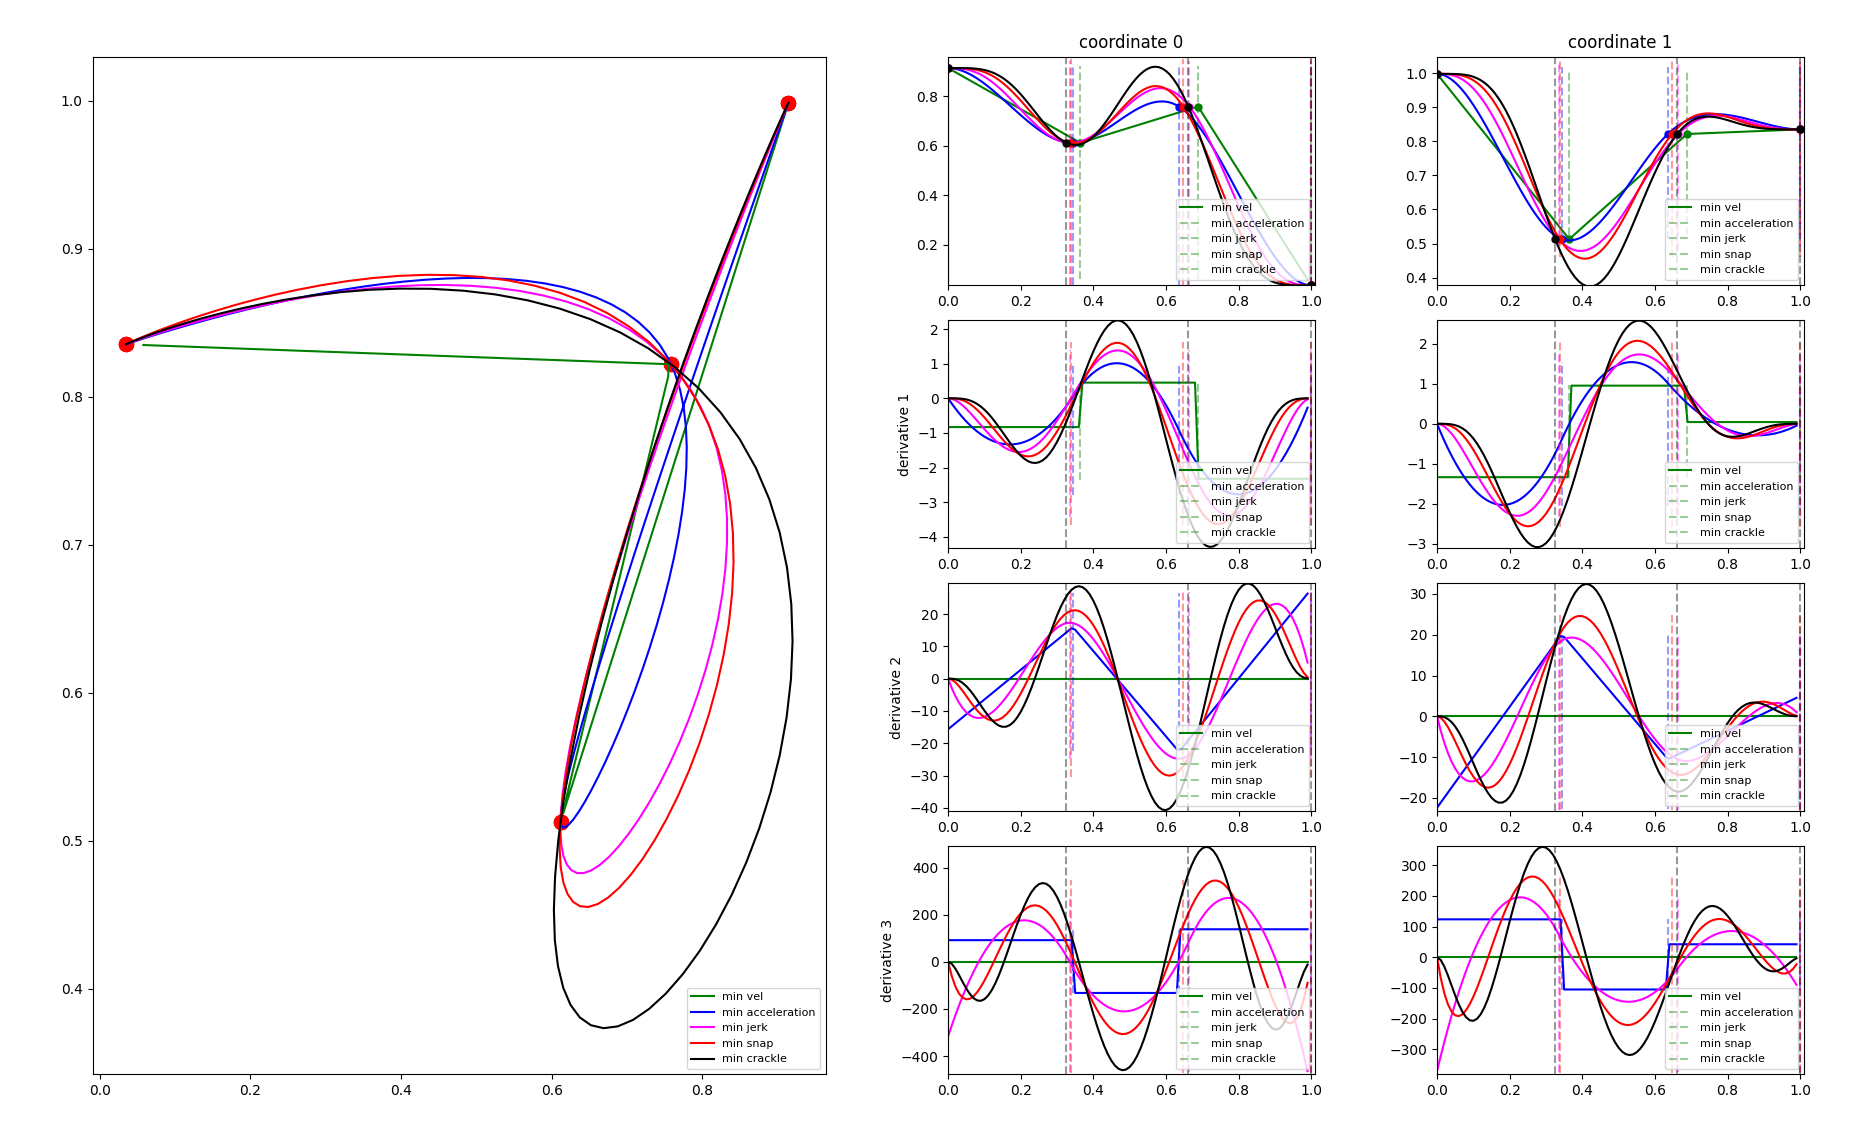
\includegraphics[width=\textwidth]{./images/comparison.png}
		\end{column}
	\end{columns}

\end{frame}

\begin{frame}[fragile]
	\frametitle{Optimization: Parametriuation Generation.}
	\framesubtitle{Minimum time stop for collision avoidance}
	\begin{columns}
		\begin{column}{0.4\textwidth}
			\begin{lstlisting}[language=python,
            ]
import gsplines
import gsplines.plot as gplot
import numpy as np
import opstop
from gsplines.optimization import minimum_jerk_path


model_file = 'path_to_urdf_robot_description'

dim = 7   # number of joints of the robot
# Generate a random numpy array of wayponts
# (each row is a waypoint in R^n)
number_of_waypoints = 5
waypoints = np.random.rand(number_of_waypoints, dim)
# The a minimum jerk trajectory with execution time of 5s
trj = minimum_jerk_path(waypoints).linear_scaling_new_execution_time(5.0)
# Select the time to stop as the 60% of the time.
stop_ti = trj.get_domain()[1]*0.6
# Get a parametrization that minimizes the time and  does not
# allow an increment in the acceleration larger than 50%
optimal_parametrization = opstop.minimum_time_bounded_acceleration(
    trj, stop_ti, 1.5, str(model_file), 8)
# Obtain the stopping trajectory
stop_trj = trj.compose(optimal_parametrization)
# Plot the nominal and the stopping trajectory
gplot.plot_compare([stop_trj, trj], ['red', 'blue'], [
                'Emergency Stop Trajectory',
                'Original Trajectory'], 
                _show=True, _up_to_deriv=2)
    \end{lstlisting}
		\end{column}
		\begin{column}{0.6\textwidth}
			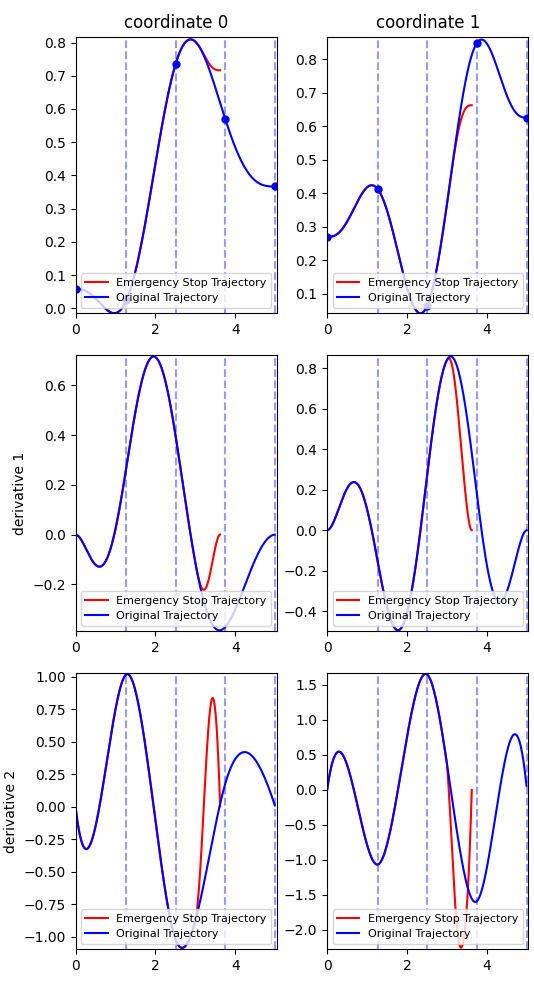
\includegraphics[width=3cm]{./images/temporal_opstopimage.png}
		\end{column}
	\end{columns}
\end{frame}

\section{Examples and comparison}
\begin{frame}[fragile]
	\frametitle{Optimization: Interface}
	\begin{columns}
		\begin{column}{0.4\textwidth}
			\begin{itemize}
				\item By balancing the jerk with the velocity we can reduce these overshoots
				      \begin{equation*}
					      \min \int_0^T \alpha \diff{\qv}{t}  + (1-\alpha) \diffk{\qv}{t}{3} \d t
				      \end{equation*}
			\end{itemize}
			\begin{lstlisting}[language=python]

waypoints = np.random.rand(4, 2)

c1 = gsplines.optimization.broken_lines_path(waypoints)
c3 = gsplines.optimization.minimum_jerk_path(waypoints)
c4 = gsplines.optimization.rojas_path(waypoints, 0.8)
c5 = gsplines.optimization.rojas_path(waypoints, 1.5)
c6 = gsplines.optimization.rojas_path(waypoints, 2)

gsplines.plot.plot2d_compare([c1, c3, c4, c5, c6], [
            'green', 'blue', 'magenta', 'red',
            'gray'],
            ['min vel', 'min jerk', 'balance k=0.8',
            'balance k=1.5', 'balance k=2'])
\end{lstlisting}
		\end{column}
		\begin{column}{0.6\textwidth}
			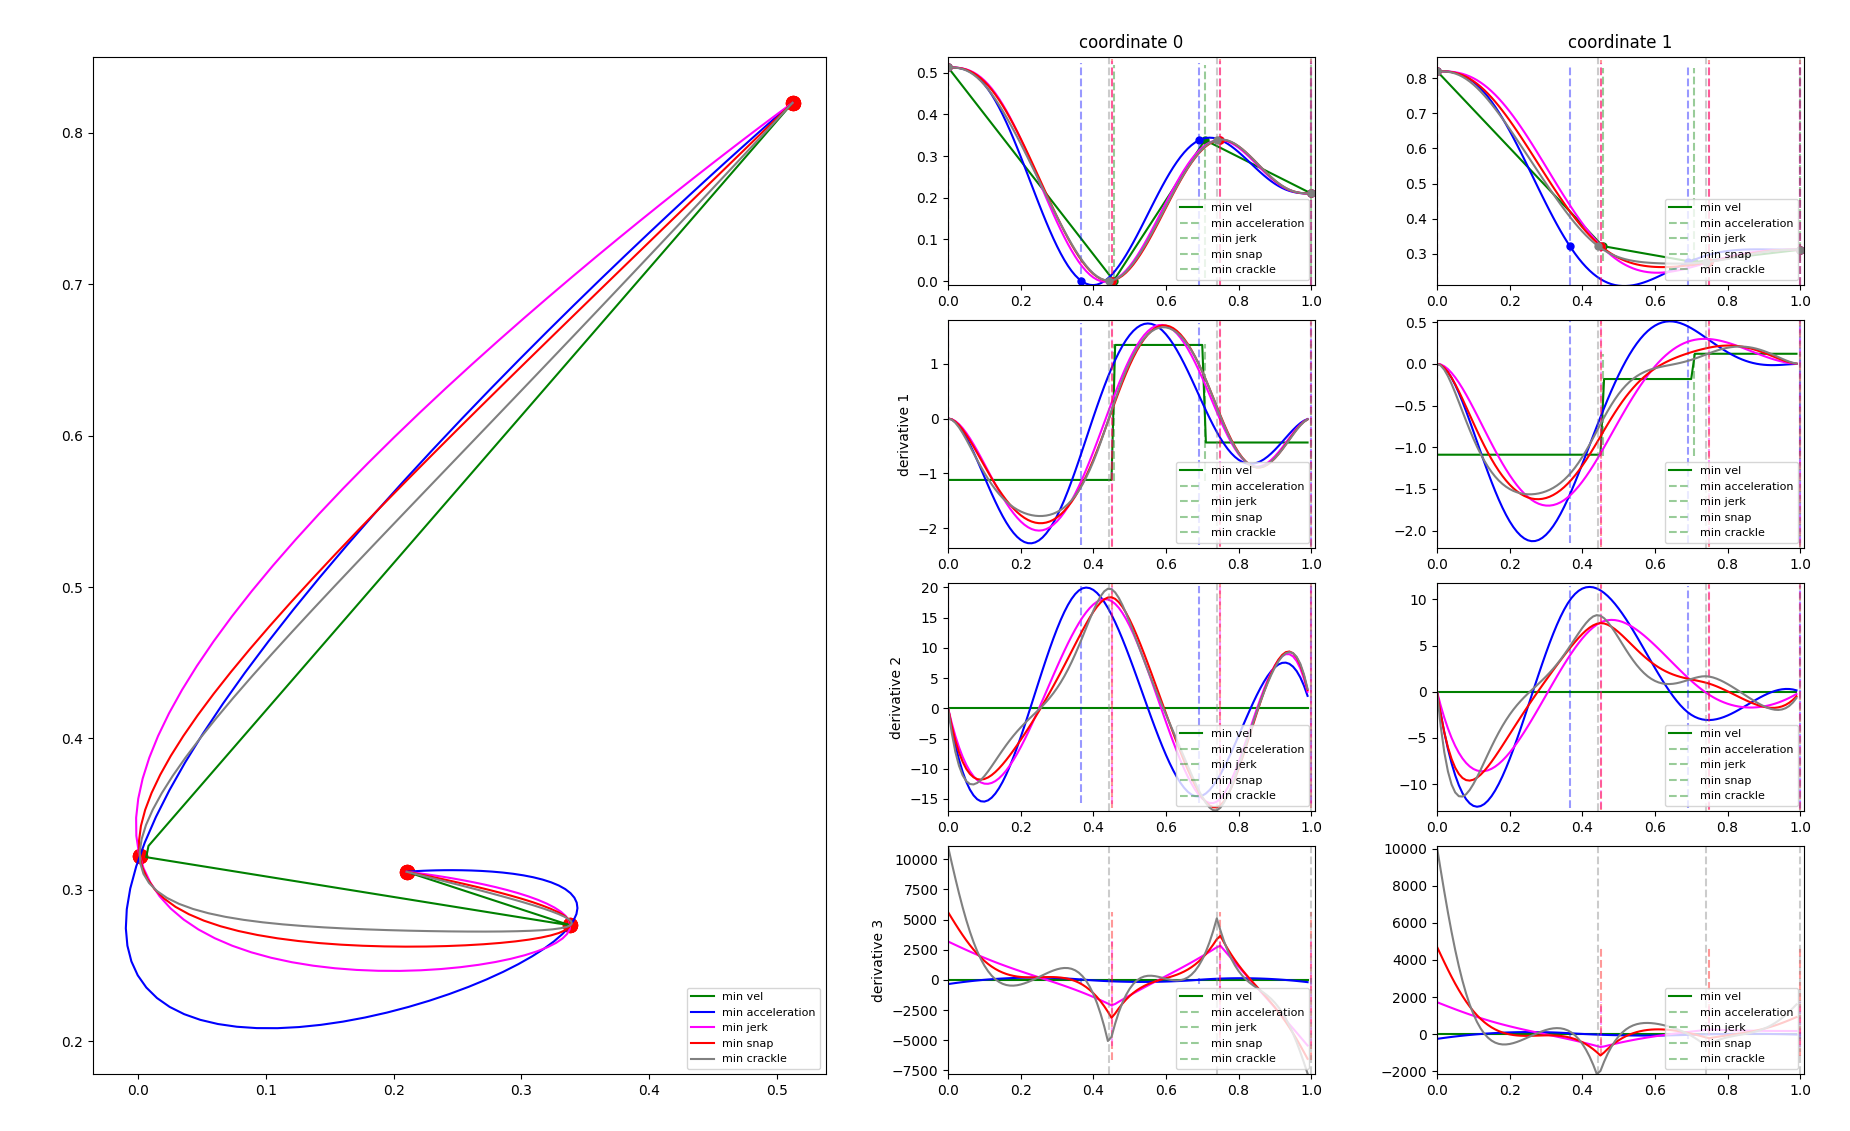
\includegraphics[width=\textwidth]{./images/comparison_2.png}
		\end{column}
	\end{columns}

\end{frame}


\begin{frame}
	\frametitle{A better type of motions}
	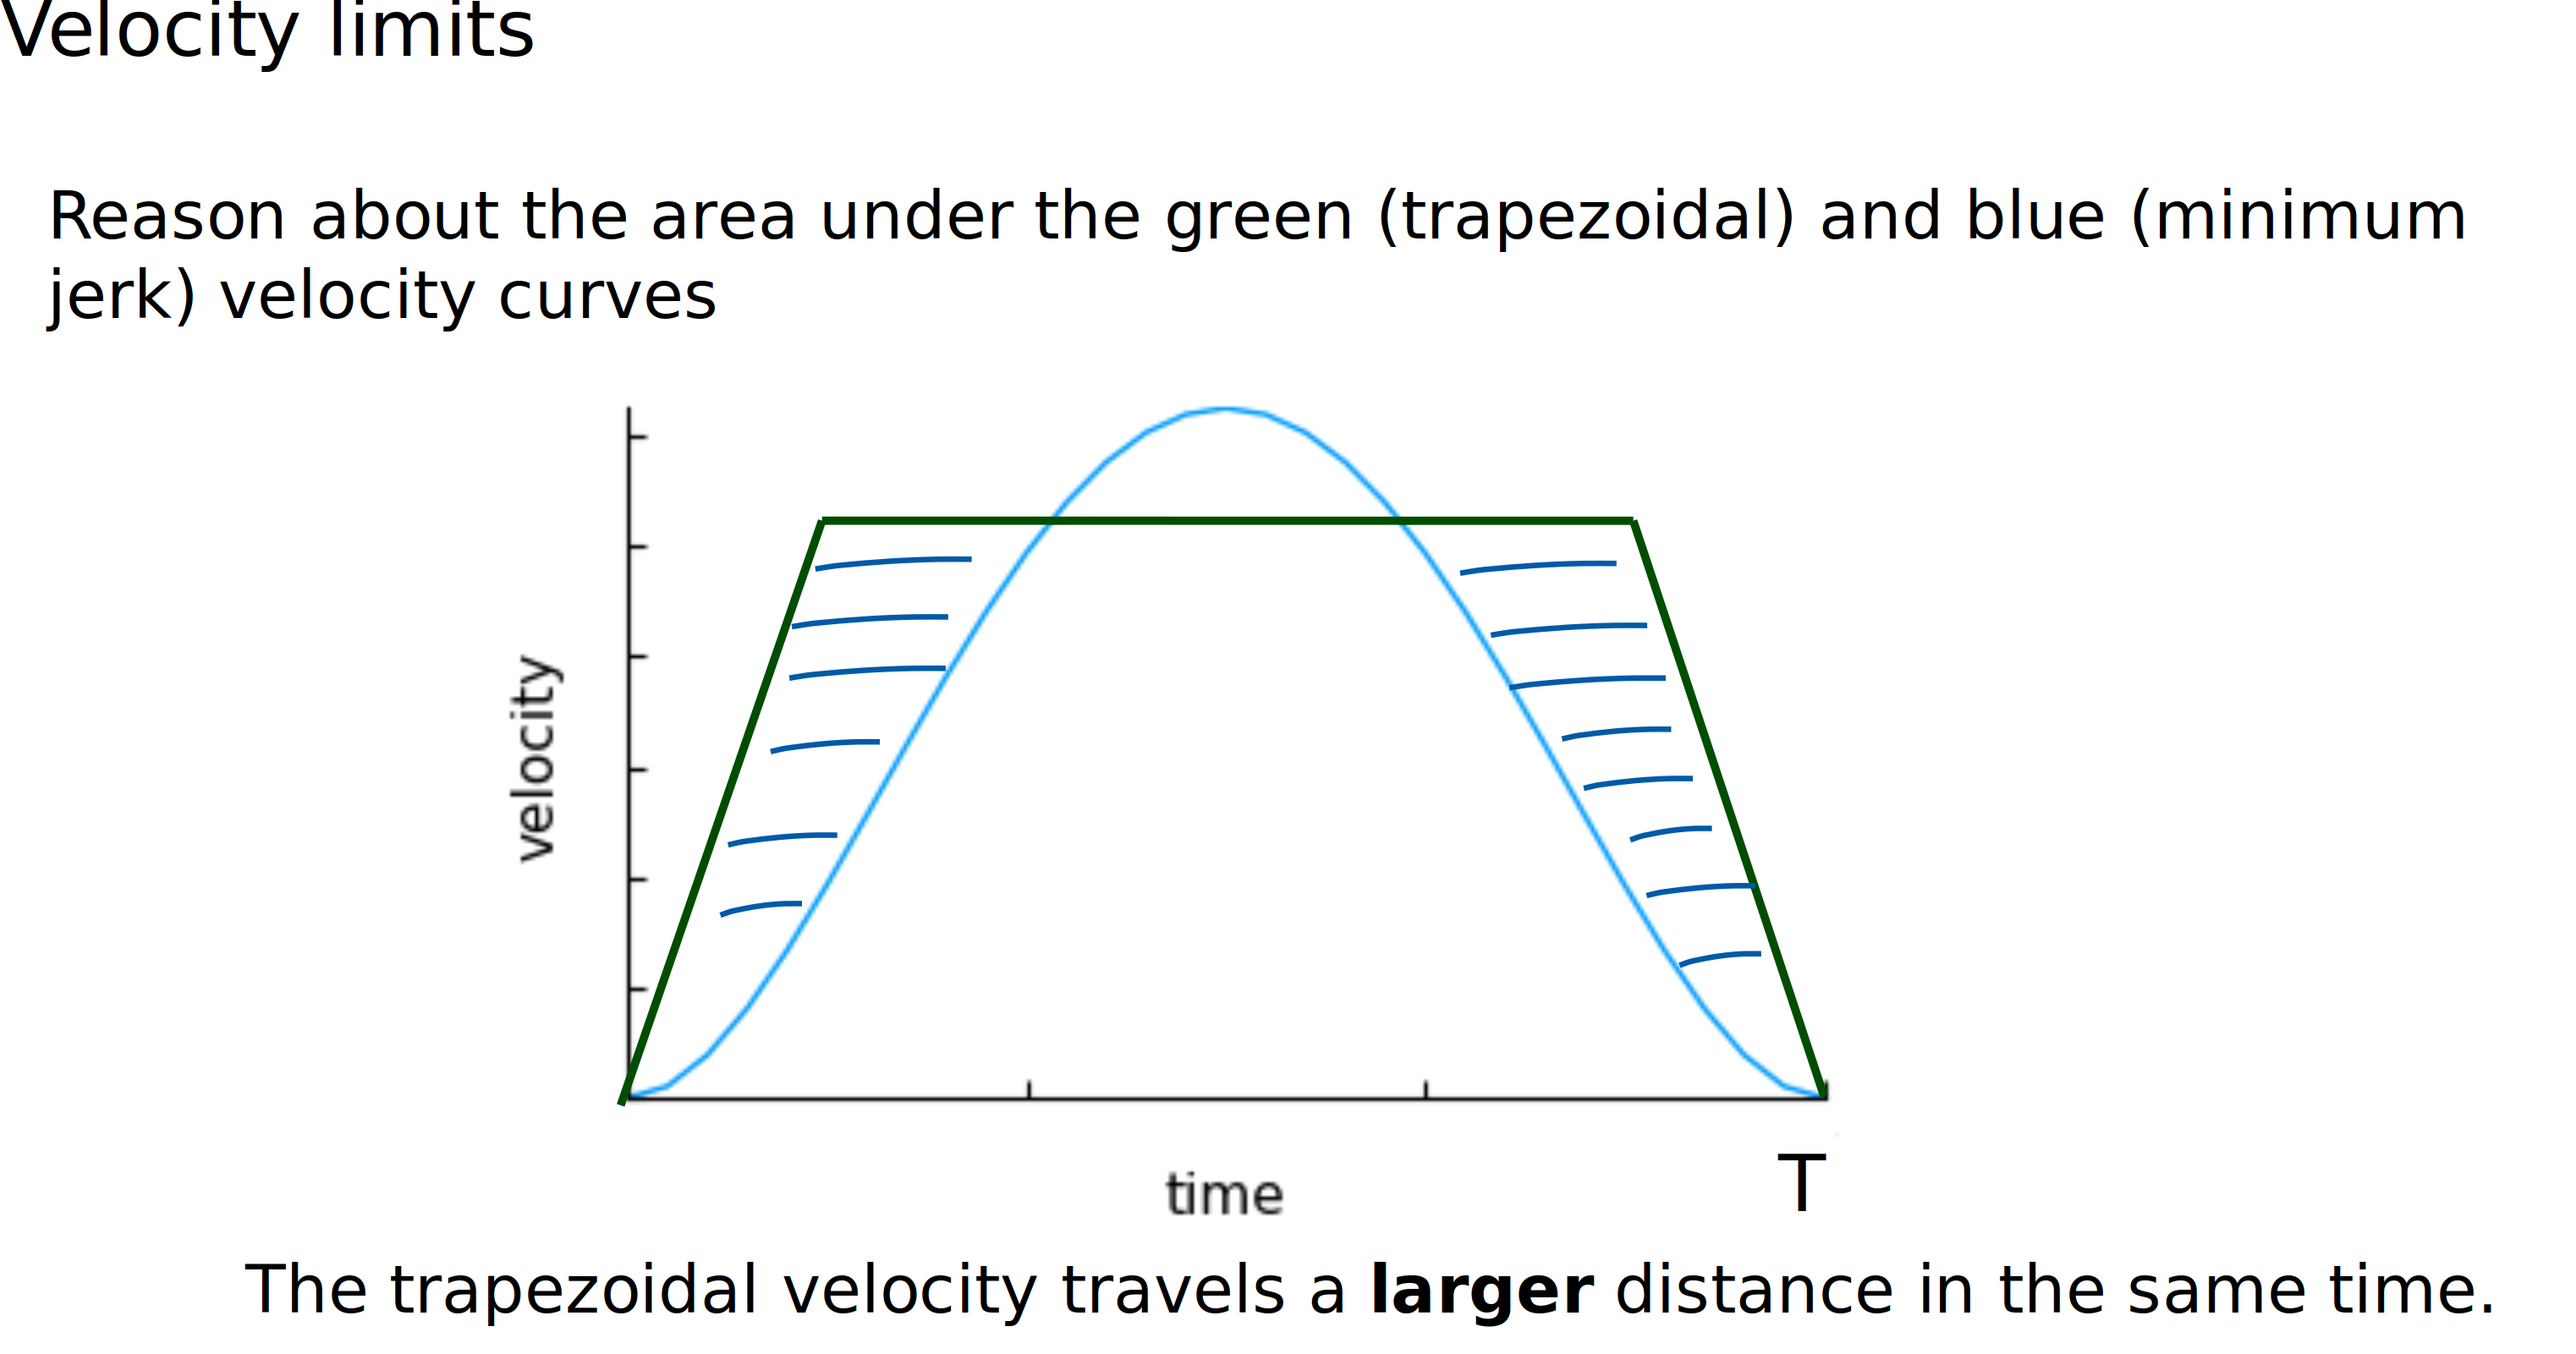
\includegraphics[width=\textwidth]{./images/temporal_slide_trapezoidal_and_corners.png}
\end{frame}

\begin{frame}
	\frametitle{Comparison with Ruckig and Pilz}
\end{frame}

\begin{frame}
	\frametitle{OpStp}
\end{frame}

\begin{frame}[fragile]
	\frametitle{Integration with ROS}
	\begin{itemize}
		\item Custom messages for \Verb|GSpline| objects: Trajectories, Basis.
		\item Conversions from \Verb|GSpline| into \Verb|trajectory_msgs::JointTrajectory| and \Verb|control_msgs::FollowJointTrajectoryGoal|
		\item Custom plot tool with \Verb|rqt| plugin based on the amasing \Verb|rqt_joint_trajectory_plot|
		\item Moveit Planner adapter \Verb|gsplines_moveit/MinimumSobolevSeminormAdapter|, can be used inside \Verb|ompl| pipeline
		      \begin{lstlisting}
gsplines_moveit/MinimumSobolevSeminormAdapter
default_planner_request_adapters/FixWorkspaceBounds
default_planner_request_adapters/FixStartStateBounds
default_planner_request_adapters/FixStartStateCollision
default_planner_request_adapters/FixStartStatePathConstraints
	          \end{lstlisting}
		\item  Controller Manager \Verb|gsplines_moveit/GSplinesControllerManager|
	\end{itemize}
\end{frame}


\begin{frame}[t]
	\frametitle{OpStop Integration}
	\begin{center}
		\begin{tikzpicture}
			\tikzumlset{font=\fontsize{5}{4}\selectfont}
			\umlbasiccomponent[x=0, y=0]{MoveGroup}
			\umlbasiccomponent[x=5]{ActionWrapper}
			\umlbasiccomponent[x=10,y=0]{ROSControl}
			\umlVHassemblyconnector[interface=FollowJointGSplineAction, anchor1=0] {MoveGroup}{ActionWrapper}
			\umlVHassemblyconnector[interface=FollowJointTrajectoryAction, anchor2=0, anchor1=180] {ROSControl}{ActionWrapper}
			\node at (MoveGroup.south) {foooooo};
		\end{tikzpicture}
	\end{center}
\end{frame}

\begin{frame}[t]
	\frametitle{OpStop Integration}
	\begin{center}
		\begin{tikzpicture}
			\begin{umlseqdiag}
				\tikzumlset{font=\fontsize{5}{4}\selectfont}
				\umlobject{MoveGroup}
				\umlobject{ActionWrapper}
				\umlobject{ROSControl}
				\begin{umlcall}[op=FollowJointGSplineGoal,return=FollowJointGSplineFeedBack]{MoveGroup}{ActionWrapper}
					\begin{umlcall}[op=FollowJointGSplineGoal,return=FollowJointTrajectoryFeedBack]{ActionWrapper}{ROSControl}
					\end{umlcall}
				\end{umlcall}
				\begin{umlcall}[op=FollowJointGSplineCancel]{MoveGroup}{ActionWrapper}
					\begin{umlcallself}[op=optimization]{ActionWrapper}{ActionWrapper}
					\end{umlcallself}
					\begin{umlcall}[op=FollowJointGSplineGoal,return=FollowJointTrajectoryFeedBack]{ActionWrapper}{ROSControl}
					\end{umlcall}
				\end{umlcall}
			\end{umlseqdiag}
		\end{tikzpicture}
	\end{center}
\end{frame}

\section{SASHA-OR}

\begin{frame}[t]
	\frametitle{SASHA-OR project}
	\framesubtitle{Situation Aware Sterile Handling Arm for the OR}
	\hglue -1cm
	\begin{tikzpicture}[scale=1, transform shape]
		\node[anchor=north west] (box) {
			\parbox{10cm}{%
				\begin{itemize}
					\item Idea
					      \begin{itemize}
						      \item \emphImFusion{Robotic scrub nurse} to address nurse shortage
						      \item Support of standardized laparoscopic interventions
					      \end{itemize}
					\item Task
					      \begin{itemize}
						      \item Handing over and receiving the required laparoscopic surgical instruments and sterile goods
					      \end{itemize}
					\item Challenges
					      \begin{itemize}
						      \item Team collaboration
						      \item Sterility maintenance
						      \item Integration into surgical workflows
						      \item Acceptance
						      \item Technical issues and reliability
					      \end{itemize}
				\end{itemize}
			}};
		\node[anchor=north west] at (box.north east) {
			\includegraphics[width=4cm]{./images/sasha-robot.jpg}};
		\node[anchor=south west] at (box.north west) {
			
\includegraphics[width=6cm]{./images/sasha-team.png}};
	\end{tikzpicture}

\end{frame}

\begin{frame}[t]
	\frametitle{SASHA-OR project}
	\framesubtitle{Situation Aware Sterile Handling Arm for the OR}
	We are interested
	\begin{itemize}
		\item Evaluate cognitive ergonomics
		      \begin{itemize}
			      \item Cognitive workload
			      \item Human perception of the motion
			      \item Human attention management
			      \item Trust and reliance
			      \item Motion preditability
		      \end{itemize}
	\end{itemize}
\end{frame}

%\begin{frame}[t]
	\frametitle{Conclusions}

\end{frame}

\begin{frame}
	\usebeamertemplate{thank you slide}
\end{frame}
\end{document}
